\begin{circuitikz}[background rectangle/.style={fill=white}, show background rectangle]
        \node(0,0) {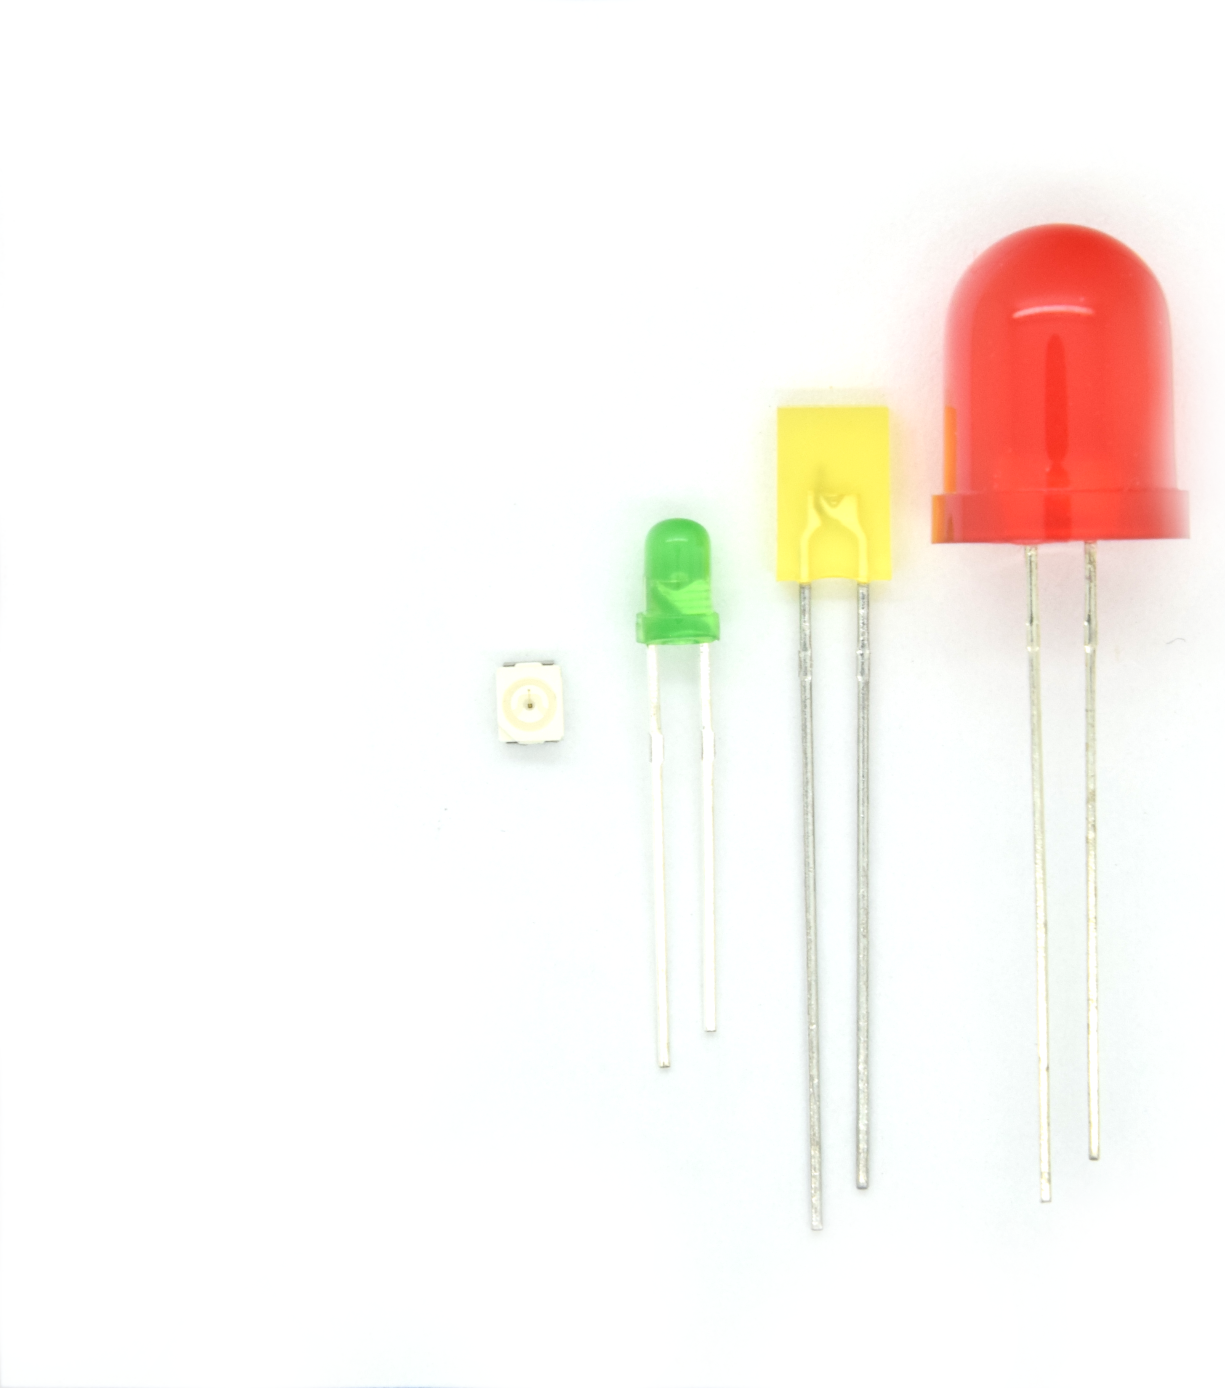
\includegraphics[width=200pt]{foto/6}};
        
        \draw(-3.0,1) to [stroke led, invert, european,l={$D$}] ++(0,-2);
    
        % Beschriftung:
        \draw( 2.50,  3.25) node {\small Rot};
        \draw( 2.50, -3.75) node {\small \qty{10}{\milli\meter}};
        \draw( 1.25,  2.00) node {\small Gelb};
        \draw( 0.35,  1.35) node {\small Grün};
        \draw( 0.35, -2.35) node {\small \qty{3}{\milli\meter}};
        \draw(-0.45,  0.50) node {\small SMD};
    
        % Pfeile:
        \draw[>=triangle 60, <->] (-1.6,0.675) coordinate(c1) -- ++(0,-1.35) coordinate(c2);
        \draw(c1) -- ++( 0.25,0);
        \draw(c1) -- ++(-0.25,0);
        \draw(c2) -- ++( 0.25,0);
        \draw(c2) -- ++(-0.25,0);
    
        % Text:
        \draw (c1) ++ (0,0.25) node {\qty{1}{\centi\meter}};
\end{circuitikz}